\documentclass{article}

\usepackage{enumitem}
\usepackage{graphicx}
\usepackage{amsmath}
\usepackage{listings}


\begin{document}
    \section{Specifica dei requisiti}
        \begin{enumerate}[label=\arabic*.]
            \item Utente
                \begin{enumerate}[label=\arabic{enumi}.\arabic*.]
                    \item nickname \{id\}
                    \item data registrazione
                    \item Venditore
                    \begin{enumerate}[label=\arabic{enumi}.\arabic{enumii}.\arabic*.]
                        \item URL
                        \item informazioni legali
                        \item possono solo vendere non comprare
                        \item popolarità = \{bassa, media, alta\}
                        \begin{enumerate}[label=\arabic{enumi}.\arabic{enumii}.\arabic{enumiii}.\arabic*.]
                            \item dipende dal NUMERO DI UTENTI che hanno effettuato negli ultimi 12 mesi bid per gli articoli da loro messi all’asta, o che hanno acquistato (sempre negli ultimi 12 mesi) articoli secondo la modalità “compralo subito”.
                            \item bassa se è inferiore a 50, media se è tra 50 e 300 e alta se è superiore a 300
                        \end{enumerate}
                    \end{enumerate}
                    \item affidabilità
                    \begin{enumerate}[label=\arabic{enumi}.\arabic{enumii}.\arabic*.]
                        \item Sia m la media aritmetica dei feedback, Sia $z$ la frazione dei feedback negativi rispetto a quelli totali allora l'affidabilità è $\frac{m(1-z)}{5}$.
                    \end{enumerate}
                \end{enumerate}
            \item Post
                \begin{enumerate}[label=\arabic{enumi}.\arabic*.]
                    \item descrizione
                    \item metodo pagamento
                    \begin{enumerate}[label=\arabic{enumi}.\arabic{enumii}.\arabic*.]
                        \item nome metodo pagamento
                        \item Bonifico oppure Carta
                    \end{enumerate}
                    \item Usato
                    \begin{enumerate}[label=\arabic{enumi}.\arabic{enumii}.\arabic*.]
                        \item può avere garanzia
                        \item condizioni = \{ottimo, buono, discreto, da sistemare\}
                    \end{enumerate}
                    \item nuovo
                    \begin{enumerate}[label=\arabic{enumi}.\arabic{enumii}.\arabic*.]
                        \item garanzia di almeno 2 anni
                    \end{enumerate}
                    \item Post che prevedono asta.
                    \begin{enumerate}[label=\arabic{enumi}.\arabic{enumii}.\arabic*.]
                        \item prezzo iniziale
                        \item ammontare dei rialzi
                        \item istante fine asta
                        \item oggetto di offerte da più utenti
                        \item operazione che indica se l'asta si è conclusa qual'è stato utente vincitore
                        \item operazione che indica il prezzo per cui è stato venduto l'oggetto nel post
                    \end{enumerate}
                    \item Post che NON prevedono asta
                    \begin{enumerate}[label=\arabic{enumi}.\arabic{enumii}.\arabic*.]
                        \item prezzo
                        \item venduti al primo cliente (utente) che ne fa richiesta
                    \end{enumerate}
                \end{enumerate}
            \item Bid
                \begin{enumerate}[label=\arabic{enumi}.\arabic*.]
                    \item istante in cui è stato proposto
                    \item utente offerente (chiamato bidder)
                    \item operazione valore proposto per quel bid.
                \end{enumerate}
            \item Categoria
                \begin{enumerate}[label=\arabic{enumi}.\arabic*.]
                    \item le categorie sono organizzate ad albero
                    \item l'albero è unito
                    \item da ogni categoria deve essere possibile ottenere le sottocategorie
                \end{enumerate}
            \item Feedback
                \begin{enumerate}[label=\arabic{enumi}.\arabic*.]
                    \item dedicato agli utenti che si aggiudicano un asta oppure se hanno comprato secondo la modalità compro-subito.
                    \item valore = 0..5
                    \item PUO' avere un commento testuale
                    \item un feedback può arrivare sia per un utente che per un venditore professionale
                \end{enumerate}
        \end{enumerate}
    \section{UML}

    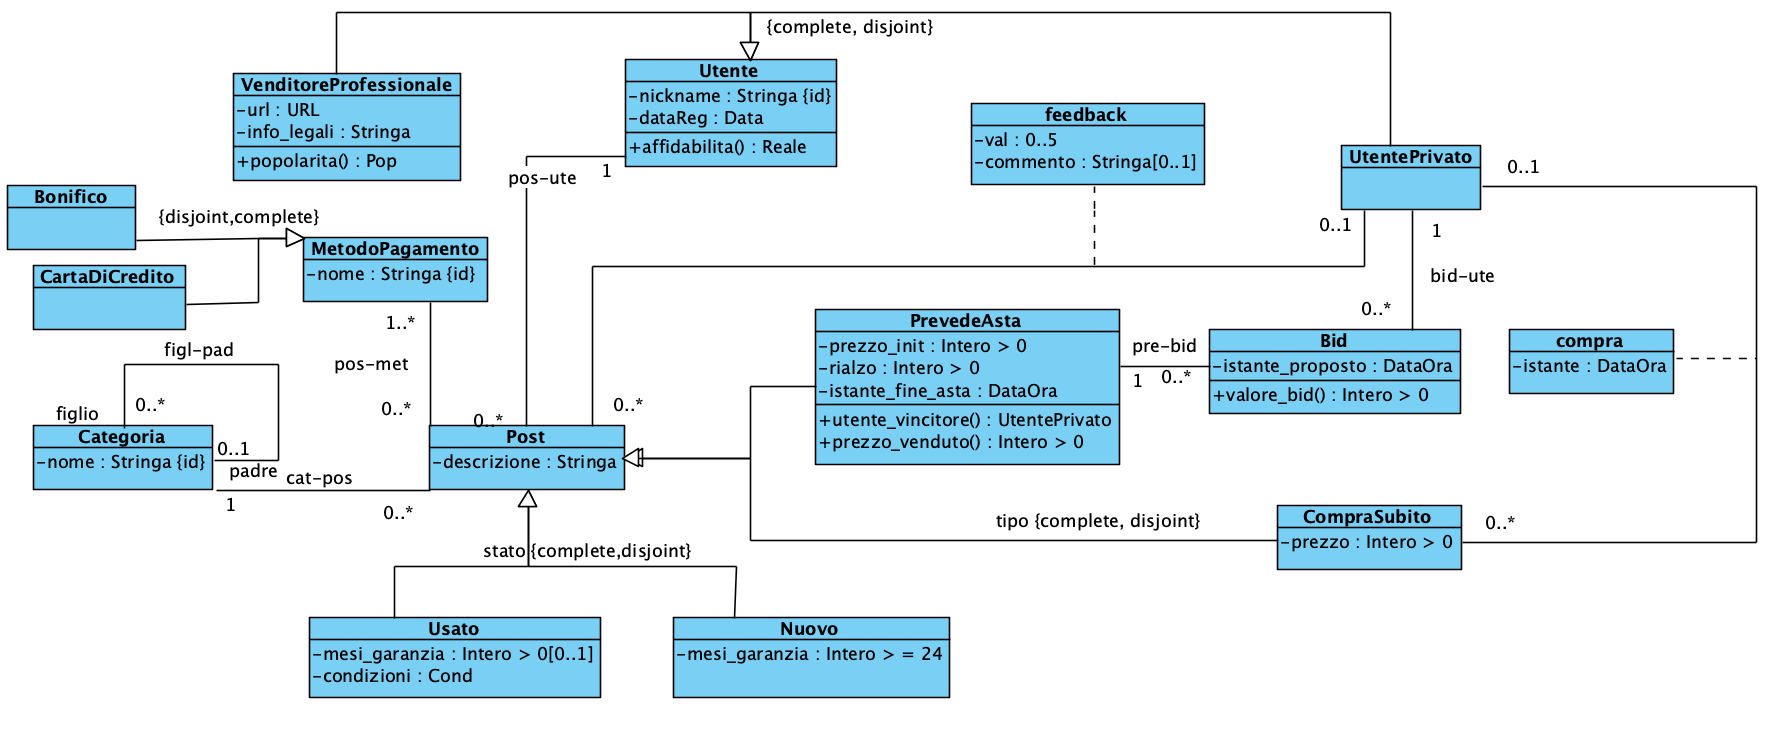
\includegraphics[width=\textwidth]{UML.png}

\section{Specifica dei vincoli}

    [V.PrevedeAsta.1]
    \[
        \forall p,b \text{ } pre-bid(p,b) \implies \\
            b.istante\_proposto < p.istante\_fine\_asta
    \]

    [V.Categoria.padreunico]
    \[
        \forall u \text{ } Categoria(u) \land \neg\exists v figl-pad(u,v) \implies \\
            \neg\exists z( z\not = u \land \neg\exists n figl-pad(z,n) )
    \]

    [V.feedback.aggiudicato]
    \begin{equation}
        \begin{gathered}
            \forall u,p feedback(u,p) \implies (\\
                PrevedeAsta(p) \implies p.istante\_fine\_asta < adesso \land p.utente\_vincitore() = u\\
                    \land\\
                CompraSubito(p) \implies compra(p,u)\\
            )
        \end{gathered}
    \end{equation}

\section{Specifica dei tipi di dato}
\begin{itemize}
 
\item tipo $Cond = {ottimo, buono, discreto, da_sistemare}$

\item tipo URL = url secondo standard

\item tipo $Pop = {bassa, media, alta}$

\end{itemize}

\section{Specifica delle classi}

\subsection{Classe Bid}

\begin{lstlisting}
    valore_bid(): intero > 0
    pre-condizioni: nessuna
    post-condizioni:
\end{lstlisting}

\begin{equation}
    \begin{gathered}
    \forall p \text{ } pre-bid(p,this) \implies (\\
        \text{sia } B = \left\{b | pre-bid(p,b) \land b.istante\_proprosto < this.istante_proposto \right\}\\
        result = |B| \cdot p.rialzo + p.prezzo\_init\\
        )
    \end{gathered}
\end{equation}

\subsection{Classe Prevede Asta}



\end{document}